%
% IAT 267: Introduction to Technological Systems - A Course Overview
%
% Author: Jeffrey Leung
%

\documentclass[10pt, oneside, letterpaper, titlepage]{article}

\usepackage{circuitikz}
\usepackage[ampersand]{easylist}
	\ListProperties(
		Progressive*=5ex,
		Space=5pt,
		Space*=5pt,
		Style1*=\textbullet\ \ ,
		Style2*=\begin{normalfont}\begin{bfseries}\textendash\end{bfseries}\end{normalfont} \ \ ,
		Style3*=\textasteriskcentered\ \ ,
		Style4*=\begin{normalfont}\begin{bfseries}\textperiodcentered\end{bfseries}\end{normalfont}\ \ ,
		Style5*=\textbullet\ \ ,
		Style6*=\begin{normalfont}\begin{bfseries}\textendash\end{bfseries}\end{normalfont}\ \ ,
		Style7*=\textasteriskcentered\ \ ,
		Style8*=\begin{normalfont}\begin{bfseries}\textperiodcentered\end{bfseries}\end{normalfont}\ \ ,
		Hide1=1,
		Hide2=2,
		Hide3=3,
		Hide4=4,
		Hide5=5,
		Hide6=6,
		Hide7=7,
		Hide8=8 )
\usepackage[T1]{fontenc}
\usepackage{geometry}
	\geometry{margin=1.2in}
\usepackage{graphicx}
	\graphicspath{ {img/} }
\usepackage[colorlinks=true, linkcolor=blue]{hyperref}
\usepackage{IEEEtrantools}
%\usepackage{lmodern} % Allows the use of symbols in font size 10; http://ctan.org/pkg/lm
\usepackage{listings}
	\lstset
	{
		breaklines=true,
		showstringspaces=false,
		language=C
	}
\usepackage[default, osfigures]{opensans}
\usepackage{siunitx}
\usepackage{textcomp}  % Allows the use of \textbullet with the font
\usepackage{tikz}
\usepackage{verbatim}

\renewcommand{\arraystretch}{1.5}
%\renewcommand{\familydefault}{\sfdefault}

\title{IAT 267: Introduction to Technological Systems \\\medskip \Large A Course Overview}
\author{Jeffrey Leung \\ Simon Fraser University}
\date{Spring 2016}

\begin{document}

	\hypersetup{pageanchor=false}
	\maketitle
	\tableofcontents3
	\clearpage
	\hypersetup{pageanchor=true}

	%
% IAT 267: Introduction to Technological Systems - A Course Overview
% Section: Introduction to Embedded and Computing Systems
%
% Author: Jeffrey Leung
%

\section{Introduction to Embedded and Computing Systems}
	\label{sec:introduction-to-embedded-and-computing-systems}
\begin{easylist}

	& \emph{Hardware:} Physical components of a digital system
	& \emph{Software:} Electronically stored instructions of a digital system

	& \emph{Embedded system:} System which interacts with another system and/or other components
		&& Components:
			&&& \emph{Microprocessor:} CPU combined with an integrated circuit
			&&& \emph{Sensor:} Device which converts a measured physical quantity into a signal
			&&& \emph{Actuator:} Mechanical device for moving/controlling a mechanism/systems

	& \emph{Computing system:}
		&& Purpose is to convert data to information

		&& Operations:
			&&& Input/output
				&&&& Communication to send/receive data
			&&& Storage (permanent/temporary)
			&&& Processing to transform data to information

		&& Main concepts:

			&&& \emph{Theory of the Universal Computing Device:} Given enough time and memory, all computers are capable of computing the same operations
			
			&&& \emph{Turing machine:} Mathematical model of a device which can perform any computation using discrete states and transitions between states
				&&&& Idea created by Alan Turing
				&&&& Ability to read and write symbols on an infinite `tape' (memory)
				&&&& \emph{Universal Turing Machine:} Machine which can implement all Turing machines
					&&&&& Programmable; instructions may be part of the input data
					&&&&& Can be emulated by a computer
				&&& E.g. Two computers A and B which have instructions which can add two values or produce the negative of a value, but B alone can subtract two values. A and B can compute the same operations.

			&&& Break-down of the levels of a computing system:
				&&&& Levels (high-level to low-level):
					&&&&& Natural language:
						&&&&&& May be ambiguous and imprecise
					&&&&& Algorithm:
						&&&&&& Step-by-step procedure
						&&&&&& Well-defined
						&&&&&& Finite
						&&&&&& Effective computability
					&&&&& Programming language:
						&&&&&& Expression of a program using a defined language
					&&&&& Instruction set architecture (ISA)
					&&&&& Microarchitecture:
						&&&&&& Organization of a processor implementation
						&&&&&& Implements a single ISA
					&&&&& Circuit:
						&&&&&& Combination of different structures to represent microarchitecture
					&&&&& Device:
						&&&&&& E.g. Capacitors, resistors, transistors
				&&&& Transformations between levels:
					&&&&& \emph{Software design:} Expression of a problem in a natural language with algorithms and data structures
					&&&&& \emph{Programming:} Implementation of algorithms and data structures using a programming language(s)
					&&&&& \emph{Compilation/interpretation:} Transformation of a program in a programming language into the instructions (in machine language) of a given instruction set
					&&&&& Circuits are created with small components such as gates

\end{easylist}
\clearpage

	%
% IAT 267: Introduction to Technological Systems - A Course Overview
% Section: Electricity and Circuit Design
%
% Author: Jeffrey Leung
%
\section{Electricity and Circuit Design}
	\label{sec:electricity-and-circuit-design}
\subsection{Electricity}
	\label{subsec:electricity-and-circuit-design:electricity}
\begin{easylist}

	& \emph{Voltage:} Relative level of electrical energy between any two given points in a circuit
		&& Denoted by \si{\volt}
		&& SI unit: Volts (\si{\volt})
		&& Totals 0 over the entire circuit
			&&& Power sources add to the voltage; components subtract from the voltage
	& \emph{Current:} Amount of electrical energy passing through any given point in a circuit
		&& Denoted by I
		&& SI unit: Amperes/amps (\si{\ampere})
		&& Constant throughout the circuit
		&& Follows the path of least resistance

	& \emph{Resistance:} Amount of difficulty in moving an electric current through a given component
		&& Denoted by R
		&& SI unit: Ohms (\si{\ohm})
		&& Inherent property of a material
		&& \emph{Conductor:} Material which has a low resistance
		&& \emph{Insulator:} Material which has a high resistance
		&& Calculating resistance:
			&&& \hyperref[subsec:electricity-and-circuit-design:circuits]{Series circuit}: Add the individual resistances

			&&&& Formula:

			\begin{displaymath}
				R_{T}
				= \sum_{i=0}^{n} R_{i}
			\end{displaymath}

			&&&& E.g. For the circuit in figure~\ref{fig:series-circuit-total-resistance-example},

			\begin{figure}[!htb]
				\begin{center}
					\begin{circuitikz}
						\draw (0,0)
						to [battery] (0, 3)
						to [R, l=R1 (820\ \si{\ohm})] (3, 3)
						to [R, l=R2 (1200\ \si{\ohm})] (3, 0)
						to [R, l=R3 (150\ \si{\ohm})] (0, 0);
					\end{circuitikz}
				\end{center}
					\caption{Series circuit with resistors 820 \si{\ohm}, 1200 \si{\ohm}, 150 \si{\ohm}}
					\label{fig:series-circuit-total-resistance-example}
			\end{figure}

			The total resistance is:
			\Deactivate
			\begin{IEEEeqnarray}{ r C l }
				R_{T}
				& = & \sum_{i=0}^{n} R_{i} \\
				& = & R_{1} + R_{2} + R_{3} \\
				& = & 820\ \si{\ohm} + 1200\ \si{\ohm} + 150\ \si{\ohm} \\
				& = & 2170\ \si{\ohm}
			\end{IEEEeqnarray}
			\Activate

			&&& \hyperref[subsec:electricity-and-circuit-design:circuits]{Parallel circuit}: Find the current of each individual path (see \emph{Ohm's Law} below) (voltage is constant throughout the circuit), and divide the voltage by the sum of the resulting currents

				&&&& Formula:

				\begin{displaymath}
					R_{T}
					= \frac{V}{\sum^{n}_{i=0} \frac{V}{R_{i}}}
					= \frac{1}{\sum^{n}_{i=0} \frac{1}{R_{i}}}
				\end{displaymath}

				&&&& E.g. For the circuit in figure~\ref{fig:parallel-circuit-total-resistance-example-1},

				\begin{figure}[!htb]
					\begin{center}
						\begin{circuitikz}
							\draw (0,0)
							to [battery, l=60\ \si{\volt}] (0,3)
							to [short] (9,3)
							to [R, l_=R3 (20 \si{\ohm})] (9,0)
							to [short] (0,0);

							\draw (6,3)
							to [R, l_=R2 (12 \si{\ohm})] (6,0);

							\draw (3,3)
							to [R, l_=R1 (6 \si{\ohm})] (3,0);
						\end{circuitikz}
					\end{center}
					\caption{Parallel circuit with resistors 6 \si{\ohm}, 12 \si{\ohm}, 20 \si{\ohm}}
					\label{fig:parallel-circuit-total-resistance-example-1}
				\end{figure}

				The currents are:

				\begin{displaymath}
					I_{1}
					= \frac{V_{1}}{R_{1}}
					= \frac{60\ \si{\volt}}{6\ \si{\ohm}}
					= 10\ \si{\ampere}
				\end{displaymath}

				\begin{displaymath}
					I_{2}
					= \frac{V_{2}}{R_{2}}
					= \frac{60\ \si{\volt}}{12\ \si{\ohm}}
					= 5\ \si{\ampere}
				\end{displaymath}

				\begin{displaymath}
					I_{3}
					= \frac{V_{3}}{R_{3}}
					= \frac{60\ \si{\volt}}{20\ \si{\ohm}}
					= 3\ \si{\ampere}
				\end{displaymath}

				\begin{displaymath}
					I_{T}
					= \sum_{i=0}^{n} I_{i}
					= I_{1} + I_{2} + I_{3}
					= 10\ \si{\ampere} + 5\ \si{\ampere} + 3\ \si{\ampere}
					= 18\ \si{\ampere}
				\end{displaymath}

				Therefore, the total resistance is:

				\begin{displaymath}
					R_{T}
					= \frac{\si{\volt}_{T}}{I_{T}}
					= \frac{60\ \si{\volt}}{18\ \si{\ampere}}
					= 3.\overline{3}\ \si{\ohm}
				\end{displaymath}

				&&&& E.g. For the circuit in figure~\ref{fig:parallel-circuit-total-resistance-example-2},

				\begin{figure}[!htb]
					\begin{center}
						\begin{circuitikz}
							\draw (0,0)
							to [battery, l=60\ \si{\volt}] (0,3)
							to [short] (9,3)
							to [R, l_=R3 (10 \si{\ohm})] (9,0)
							to [short] (0,0);

							\draw (6,3)
							to [R, l_=R2 (15 \si{\ohm})] (6,0);

							\draw (3,3)
							to [R, l_=R1 (5 \si{\ohm})] (3,0);
						\end{circuitikz}
					\end{center}
					\caption{Parallel circuit with resistors 5 \si{\ohm}, 15 \si{\ohm}, 10 \si{\ohm}}
					\label{fig:parallel-circuit-total-resistance-example-2}
				\end{figure}

				The total resistance is:

				\Deactivate
				\begin{IEEEeqnarray}{ r C l }
					R_{T}
					& = & \frac{1}{ \sum_{i=0}^{n} \frac{1}{R_{i}} } \\
					& = & \frac{1}{ \frac{1}{R_{1}} + \frac{1}{R_{2}} + \frac{1}{R_{3}} } \\
					& = & \frac{1}{ \frac{1}{5} + \frac{1}{15} + \frac{1}{10} } \\
					& = & \frac{1}{ \frac{6}{30} + \frac{2}{30} + \frac{3}{30} } \\
					& = & \frac{1}{ \frac{11}{30} } \\
					& = & \frac{30}{11}\ \si{\ohm}
				\end{IEEEeqnarray}
				\Activate

	& \emph{Ohm's Law:} Formula relating voltage, current, and resistance
		&& Formula:

		\begin{displaymath}
			V = I \cdot R
		\end{displaymath}

		\medskip

		\begin{center}
			\Deactivate
			\begin{tabular}{ l r @{ = } l }
				where
				& $V$ & Voltage \\
				& $I$ & Current \\
				& $R$ & Resistance
			\end{tabular}
			\Activate
		\end{center}

		&& \emph{Short-circuit:} Insufficient resistance which creates too much current (as voltage is constant), damaging the circuit

	\bigskip

	& \emph{Power:} Rate at which electrical energy is transferred
		&& Denoted by P
		&& SI unit: Watt (\si{\watt})
		&& Formula:

		\begin{displaymath}
			P = V \cdot I
		\end{displaymath}

		\begin{center}
			\Deactivate
			\begin{tabular}{ l r @{ = } l }
				where
				& $P$ & Power \\
				& $V$ & Voltage \\
				& $I$ & Current
			\end{tabular}
			\Activate
		\end{center}

	& Electron flow:
		&& From greater electrical energy to lesser electrical energy
		&& From the negative terminal to the positive terminal

\end{easylist}
\subsection{Types of Electricity}
	\label{subsec:electricity-and-circuit-design:types-of-electricity}
\begin{easylist}

	& \emph{Piezoelectricity:} Electrical potential created from pressure energy exerted upon a polarized crystal
		&& Discovered in 1880s by the Curies
		&& Explanation:
			&&& Piezoelectric crystals are permanently electrically polarized, aligning the dipoles and attracting excess surface charge to electrically neutralize the crystal
			&&& Applying force to the piezoelectric crystal disrupts the orientation of electric dipoles which creates temporary excess charge
		&& E.g. Quartz is compressed to create a consistent electrical signal in a watch
		&& For applications, see \hyperref[sec:sensors]{Sensors} and \hyperref[sec:actuators]{Actuators}

\end{easylist}
\subsection{Circuits}
	\label{subsec:electricity-and-circuit-design:circuits}
\subsubsection{Introduction}
	\label{subsubsec:electricity-and-circuit-design:circuits:introduction}
\begin{easylist}

	& \emph{Circuit:} Loop of electronic components with a power source and a load

	& Input pins not grounded or connected to power may exhibit variable capacitance (electrical energy)
		&& Example of proper grounding: See figure~\ref{fig:example-input-pin-grounding}

		\begin{figure}[!htb]
			\begin{center}
				\begin{circuitikz}
					\draw (0, 6)
					to [closing switch] (0, 4)
					to [R, l_=10k\ \si{\ohm}] (0, 2)
					to (0, 2) node[ground]{};

					\draw (0, 4)
					to [short, l=Input\ pin] (2, 4);
				\end{circuitikz}
			\end{center}
				\caption{Example of Input Pin Grounding}
				\label{fig:example-input-pin-grounding}
		\end{figure}

	& \emph{Schematic:} Visual representation of a system using standardized symbols

\end{easylist}
\subsubsection{Components}
	\label{subsubsec:electricity-and-circuit-design:circuits:components}
\begin{easylist}

	& \emph{Power source:} Provider of electrical energy
		&& Denoted by:

			&&& Voltage source (American):
			\begin{center}
				\begin{circuitikz}
					\draw (0,0)
					to [american voltage source] (2,0);
				\end{circuitikz}
			\end{center}

			&&& Battery:
			\begin{center}
				\begin{circuitikz}
					\draw (0,0)
					to [battery] (2,0);
				\end{circuitikz}
			\end{center}

				&&&& Longer line is the positive terminal; shorter line is the negative terminal

		&& E.g. Battery, wall plug

	& \emph{Electrical load:} Component which consumes electrical energy
		&& E.g. Light bulb

	& \emph{Resistor:} Electrical component which limits the current in a circuit
		&& Denoted by:
		\begin{center}
			\begin{circuitikz}
				\draw (0,0)
				to [R] (2,0);
			\end{circuitikz}
		\end{center}

		&& \emph{Potentiometer:} Resistor which has adjustable/variable resistance
			&&& Denoted by:
			\begin{center}
				\begin{circuitikz}
					\draw (0,0)
					to [pR] (2,0);
				\end{circuitikz}
			\end{center}
			&&& Connections:
				&&&& Side prong to positive
				&&&& Middle prong to output
				&&&& (Other) side prong to ground
				&&&& Turning the knob moves the middle prong along a resistor, closer/farther to the side prong, forcing the current to move through greater resistance

	& \emph{Polarization:} Characteristic of an electrical component which only operates when the current flows in a specific direction
		&& Anode (longer prong) is connected to the positive terminal
		&& Cathode (shorter prong) is connected to the negative terminal

		\medskip

		&& \emph{Diode:} Electrical component which limits the flow of electricity to only one direction
			&&& Denoted by:
			\begin{center}
				\begin{circuitikz}
					\draw (0,0)
					to [Do] (2,0);
				\end{circuitikz}
			\end{center}

			&&& \emph{Light Emitting Diode (LED):} Diode which emits light when current flows through with the correct voltage
				&&&& Denoted by:
				\begin{center}
					\begin{circuitikz}
						\draw (0,0)
						to [D*] (2,0);
					\end{circuitikz}

					\medskip
					or
					\medskip

					\begin{circuitikz}
						\draw (0,0)
						to [leDo] (2,0);
					\end{circuitikz}
				\end{center}


	& \emph{Capacitor:} Electrical component which stores then releases electrical energy in intervals
		&& May be polarized
		&& Denoted by:

			&&& Unpolarized:
				\begin{center}
					\begin{circuitikz}
						\draw (0,0)
						to [capacitor] (2,0);
					\end{circuitikz}
				\end{center}

			&&& Polarized:
				\begin{center}
					\begin{circuitikz}
						\draw (0,0)
						to [polar capacitor] (2,0);
					\end{circuitikz}
				\end{center}


	& \emph{Switch:} Electrical component which controls a break in a circuit and therefore electrical energy flow
		&& Denoted by:
		\begin{center}
			\begin{circuitikz}
				\draw (0,0)
				to [closing switch] (2,0);
			\end{circuitikz}
		\end{center}

		&& Closing a switch completes the circuit; opening a switch breaks the circuit

	& \emph{(Solderless) Breadboard:} Base on which circuits can be built
		&& Useful for prototyping or designing a circuit
		&& Components should not be added or removed while the circuit is live to avoid short circuits or shocks

	& \emph{Microcontroller:} Small computer with a processor, memory, and programmable inputs/outputs

	& \emph{Analog-to-digital converter}: Device which converts an analog voltage to a digital value

\end{easylist}
\subsubsection{Types of Circuits}
	\label{subsubsec:electricity-and-circuit-design:circuits:types-of-circuits}
\begin{easylist}

	& \emph{Serial circuit:} Circuit in which all components are connected in-line
		&& I.e. Only one path exists from the positive terminal to the negative terminal for the electrons to flow through
		&& E.g. See figure~\ref{fig:series-circuit-example}.

		\begin{figure}[!htb]
			\begin{center}
				\begin{circuitikz}
					\draw (0,0)
					to [battery] (0,2)
					to [lamp] (4,2)
					to [short] (4,0)
					to [lamp] (0,0);
				\end{circuitikz}
				\caption{Example of a series circuit}
				\label{fig:series-circuit-example}
			\end{center}
		\end{figure}

		&& To find the total resistance, see \hyperref[subsec:electricity-and-circuit-design:electricity]{Calculating resistance}

	& \emph{Parallel circuit:} Circuit in which not all components are placed in-line with each other
		&& I.e. Multiple paths exist from the positive terminal to the negative terminal for the electrons to flow through
		&& E.g. See figure~\ref{fig:parallel-circuit-example}.

		\begin{figure}[!htb]
			\begin{center}
				\begin{circuitikz}
					\draw (0,0)
					to [battery] (0,2)
					to [short] (4,2)
					to [lamp] (4,0)
					to [short] (0,0);

					\draw (2,0)
					to [lamp] (2,2);
				\end{circuitikz}
				\caption{Example of a parallel circuit}
				\label{fig:parallel-circuit-example}
			\end{center}
		\end{figure}

		&& To find the total resistance, see \hyperref[subsec:electricity-and-circuit-design:electricity]{Calculating resistance}

	& \emph{Voltage divider:} Portion of a circuit which connects to the ground, using a variable resisitance from a sensor to manipulate the voltage outputted to a component
		&& For an example schematic, see figure~\ref{fig:example-voltage-divider}

		\begin{figure}[!htb]
			\begin{center}
				\begin{circuitikz}
					\draw (0, 6)
					to [short, l^=$V_{in}$] (2, 6)
					to [R, l_=$R_{1}$] (2, 4)
					to [short, l^=$V_{out}$] (4, 4);

					\draw (2, 4)
					to [R, l_=$R_{2}$] (2, 2)
					to (2, 2) node[ground]{};
				\end{circuitikz}
			\end{center}
				\caption{Example of a Voltage Divider}
				\label{fig:example-voltage-divider}
		\end{figure}

		&& Formula for output voltage:

		\begin{displaymath}
			V_{out} = \frac{R_{2}}{R_{1} + R_{2}} \cdot V_{in}
		\end{displaymath}

			&&& Explanation:

			\Deactivate
			\begin{IEEEeqnarray}{ r C l }
				V_{in}
				& = & I \cdot R \\
				& = & I \cdot (R_{1} + R_{2}) \rule[-1.5em]{0pt}{1em} \\
				I
				& = & \frac{V_{in}}{R_{1} + R_{2}} \rule[-1.5em]{0pt}{1em} \\
				V_{out}
				& = & I \cdot R \\
				& = & I \cdot R_{2} \\
				& = & \frac{V_{in}}{R_{1} + R_{2}} \cdot R_{2} \\
				& = & \frac{R_{2}}{R_{1} + R_{2}} \cdot V_{in}
			\end{IEEEeqnarray}
			\Activate

			Reminders: \\
			Voltage is the potential difference between a component in the circuit and the ground. \\
			Current ($I$) is constant throughout the circuit.

\end{easylist}
\clearpage

	%
% IAT 267: Introduction to Technological Systems - A Course Overview
% Section: Sensors
%
% Author: Jeffrey Leung
%

\section{Sensors}
	\label{sec:sensors}
\subsection{Introduction}
	\label{subsec:sensors:introduction}
\begin{easylist}

	& \emph{Sensor:} Device which converts physical information into an electrical signals
	& May output variable resistance/voltage/capacitance/current

	& Types of sensors:
		&& \hyperref[subsec:technological-systems:categories]{Analog} sensors
			&&& Examples: Rotation, slider, temperature, touch, force, light
			&&& Often provides variable resistance
		&& \hyperref[subsec:technological-systems:categories]{Digital} sensors
		&& \emph{Passive sensor:} Sensor which requires its own power source to send a signal
		&& \emph{Active sensor:} Sensor which produces its own electrical signal through sensing
			&&& E.g. Piezoelectric, thermoelectric, or radioactive sensors

	& Physical design:
		&& \hyperref[subsec:electricity-and-circuit-design:types-of-electricity]{Piezoelectricity} can be used to measure force, flexure, acceleration, heat, acoustic vibrations (microphones)

\end{easylist}
\subsection{Characteristics to Sense}
	\label{subsec:sensors:characteristics-to-sense}
\subsubsection{Orientation}
	\label{subsubsec:sensors:characteristics-to-sense:orientation}
\begin{easylist}

	& \emph{Degree of freedom:} Axis along which an object is oriented
		&& E.g. In 3-d space, x/y/z are the 3 degrees of freedom
	& Rotation terminology:
		&& X-axis: Pitch/tilt
		&& Y-axis: Pan/yaw
		&& Z-axis: Roll

\end{easylist}
\subsubsection{Presence}
	\label{subsubsec:sensors:characteristics-to-sense:presence}
\begin{easylist}

	& Binary (present vs. not present)
	& Switches:
		&&& \emph{Foot switch:} Sensor which detects the binary presence of an object by contacting metal tape placed between foam spacers when pressure is applied
			&&&& Useful for small areas
		&&& \emph{Photoelectric switch:} Sensor which detects the binary presence of an object by detecting whether an object blocks the area between a light source and the sensor
		&&& \emph{Magnetic/reed switch:} Sensor which detects the binary presence of a magnetic field using two ferromagnetic contacts which connect in the presence of a magnetic object

\end{easylist}
\subsubsection{Position}
	\label{subsubsec:sensors:characteristics-to-sense:position}
\begin{easylist}

	& May be absolute or relative
	& \emph{Ranging sensor:} Sensor which detects the distance of an object relative to the sensor by sending a signal and comparing the energy reflected back to the original energy, or by detecting the time for the signal to reflect
		&& Constrained by distance, field of view, sweet-spot zones, and interference from other sensors
			&&& Solution: Constrain the environment (e.g. number of people, number of entrances or exits) rather than using more complex/numerous sensors
		&& \emph{Infrared distance sensor:} Sensor which detects the distance of an object relative to the signal by sending an infrared signal and calculating the amount of time for the signal to reflect back
			&&& Shorter ranges than ultrasonic sensors
		&& \emph{Ultrasonic sensor:} Sensor which detects the distance of an object relative to the signal by sending an ultrasonic signal and calculating the amount of time for the signal to reflect back
			&&& Longer ranges than infrared sensors
		&& E.g. Video tracking uses ranging sensors to automatically focus the camera lens
	& Multiple distance/presence sensors can determine the exact location of an object
		&& E.g. Multiple floor switches covering an area
		&& \emph{Trilateration:} Detection of the location of an object in a space by calculating distances from various points
			&&& Multiple signals at the same time may interfere with detection, so sensors must be alternated/cycled
	& A camera on a ceiling can track an object's position

\end{easylist}
\subsubsection{Motion and Video Tracking}
	\label{subsubsec:sensors:characteristics-to-sense:motion-and-video-tracking}
\begin{easylist}

	& Motion:
		&& \emph{Motion detector:} Sensor which detects changes in the infrared light in an area
		&& Velocity/acceleration can be calculated through sensing position over time

	& Video tracking:
		&& Cameras contain thousands of photocells which detect a wide range of light
			&&& Lighting conditions must be sufficient and consistent

\end{easylist}
\subsubsection{Identity}
	\label{subsubsec:sensors:characteristics-to-sense:identity}
\begin{easylist}

	& Camera/video detection of colour/images allows for shape/pattern recognition and tracking
		&& Advantages:
			&&& Adjustable distance to object
			&&& Detection of unique features
		&& Disadvantages:
			&&& Requires line of sight
			&&& Challenging to recognize objects from any angle and lighting

	& \emph{Barcode:} 1-d rectangle of white/black lines representing a unique binary code
		&& \emph{QR (Quick Response) code:} 2-d grid of white/black squares representing a unique binary code
		&& Advantages:
			&&& Can be read from variable angles
		&& Disadvantages:
			&&& Requires line of sight
			&&& Distortion from camera to digital recognition causes errors
			&&& Must be centred

	& \emph{Radio-frequency identification (RFID):} Tracking and identification of tags attached to objects which respond to radio signals
		&& RFID reader sends a short-range radio signal to an RFID tag, which returns a string of data
		&& \emph{Passive RFID system:} RFID system which includes a radio transceiver powered by induction from the received radio signal
			&&& Requires closer proximity and is cheaper than an active RFID system
		&& \emph{Active RFID system:} RFID system which includes a radio transceiver and a power supply
			&&& Has greater distance and is more expensive than an active RFID system
		&& Advantages:
			&&& Requires proximity rather than direct line of sight
		&& Disadvantages:
			&&& Short-ranged
			&&& May experience interference from radio noise

\end{easylist}
\subsection{Examples}
	\label{subsec:sensors:examples}
\begin{easylist}

	& Rotation sensor: Variable 3-pin sensor which outputs a resistance proportional to the rotation of the dial
		&& Functions similarly to a \hyperref[subsec:electricity-and-circuit-design:circuits]{potentiometer}
	& Slider sensor: Variable 3-pin sensor which outputs a resistance proportional to the distance from one side of the slider
		&& Functions similarly to a \hyperref[subsec:electricity-and-circuit-design:circuits]{potentiometer}
	& Temperature sensor: Sensor which outputs a voltage directly proportional to the temperature
		&& Formula:
		\begin{displaymath}
			T = \frac{v-200}{4}
		\end{displaymath}

		\begin{center}
			\Deactivate
			\begin{tabular}{ l r @{ = } l }
				where
				& $T$ & Temperature (\textdegree Celsius) \\
				& $v$ & Sensor value
			\end{tabular}
			\Activate
		\end{center}

		&& \emph{Thermal resistor:} Temperature sensor which changes resistance according to temperature
			&&& \emph{Resistance temperature detector (RTD):} Thermal resistor made from a naturally occurring material (e.g. copper, nickel, platinum) which changes resistance according to temperature
			&&& \emph{Thermistor:} Thermal resistor made from an artificial material (e.g. ceramic, polymer) which changes resistance according to temperature
				&&&& Resistance is inversely proportional to temperature
		&& \emph{Thermocouple:} Temperature sensor which utilizes a voltage difference at the connection of two conductors dependent on temperature
			&&& Created by Thomas Seeback
			&&& Commonly used
			&&& Cheap
			&&& Has standard connectors
			&&& Can measure a wide range of temperatures
				&&&& Can be inaccurate
			&&& E.g. A K-type thermocouple is made from the conductors nickel-chromium and nickel-aluminum
	& Capacitive sensor: Sensor which measures the amount of electrical charge
		&& Functions through glass
		&& Stored potential energy can be increased by using larger plates

	& Force sensor: Sensor which outputs a voltage directly proportional to the amount of force applied
		&& E.g. Placing a \hyperref[subsec:electricity-and-circuit-design:types-of-electricity]{piezoelectric} crystal between two metal plates and applying pressure to the plates will create voltage directly proportional to the amount of force

		&& Force-sensing resistor: Sensor which changes resistance according to the amount of force applied
			&&& Consists of a resistive material and a set of contacts; applying force to the sensor distorts the material allowing higher conductivity (see figure~\ref{fig:diagram-force-sensing-resistor})

			\begin{figure}[!htb]
				\centering
				\href
				{http://soundlab.cs.princeton.edu/learning/tutorials/sensors/node8.html}
				{
					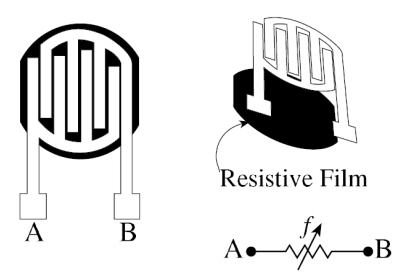
\includegraphics[scale=0.5]{force-sensing-resistor}
				}
				\caption{Diagram of a Force-Sensing Resistor}
				\label{fig:diagram-force-sensing-resistor}
			\end{figure}

		&& Flex sensor: Sensor which changes resistance according to the amount of distortion applied

		&& Pressure sensor: Sensor which measures the amount of pressure exerted by a fluid

		&& Methods to sense force:
			&&& Measurement of the acceleration of a known mass
			&&& Comparison of the unknown force against the gravitational force on the known mass (gravity-balance)
			&&& Conversion of the unknown force to a fluid pressure measured with a pressure transducer (pressure-sensing)

	& Photodetector/light sensor: Sensor which outputs a voltage proportional to the amount of light received
		&& \emph{Photodiode/quantum detector:} Light sensor which converts electromagnetic radiation into current in a semiconductor
			&&& Good detector of optical radiation
		&& \emph{Thermal detector:} Light sensor which absorbs infrared radiation and measures the \\ change in temperature

\end{easylist}
\subsection{Quality of Input}
	\label{subsec:sensors:quality-of-input}
\begin{easylist}

	& \emph{Transfer function:} Relationship/mapping of the electrical output signal by the physical input signal
		&& Calibration is done by applying known physical inputs and recording electrical outputs

	& \emph{Sensitivity:} Amount of change in output value given a change in input value
	& \emph{Accuracy:} Proximity of the measured value to the actual value
		&& Expressed as a percentage of the actual value

	& \emph{Precision:} Ability to create consistent output values within a given deviation from similar input values
	& \emph{Repeatability:} Ability to create consistent output values from a constant input value under the same environmental conditions
	& \emph{Stability:} Consistency of output values given a constant input value over a period of time
		&& Expressed as a percentage of the output
		&& Inverse of the amount of drift
		&& Reliable sensors have a drift of $< 2\%$

	& \emph{Range:} Difference between the minimum and maximum input limits/possibilities
		&& \emph{Span:} Difference between the minimum and maximum input values

	& \emph{Hysteresis:} Variation in output value for the same input value due to the change of the input value (i.e. increasing or decreasing)

	& \emph{Noise:} Fluctuations in the output values not caused by the input values
		&& May limit performance of a sensor

\end{easylist}
\clearpage

	%
% IAT 267: Introduction to Technological Systems - A Course Overview
% Section: Actuators
%
% Author: Jeffrey Leung
%

\section{Actuators}
	\label{sec:actuators}
\begin{easylist}

	& \emph{Pulse-width modulation:} Emulation of analog output using digital-only actuators by pulsing the output on and off repeatedly
		&& The magnitude of the analog output is proportional to the amount of time the output is on relative to the amount of time the output is off

\end{easylist}
\subsection{Light and Display}
	\label{subsec:actuators:light-and-display}
\begin{easylist}

	& \hyperref[subsubsec:electricity-and-circuit-design:circuits:components]{LEDs}:
		&& LED driver chip regulates the power to a matrix (grid) of LEDs

	& \emph{Liquid Crystal Display (LCD):} Display which allows for detailed display on a screen
		&& Generally use 4 or 8 pins to input data and 3 pins for communication synchronization

\end{easylist}
\subsection{Motion}
	\label{subsec:actuators:motion}
\begin{easylist}

	& Characteristics of motors:
		&& Voltage
		&& Critical current values:
			&&& \emph{Stall current:} Amount of current used when the motor is applying maximum torque due to being held in place during operation
				&&&& Highest possible current during normal operation
			&&& \emph{Running current:} Amount of current used when the motor is activated normally
		&& Speed
		&& Torque
		&& Position (servos/steppers only)
	& Types of motors:
		&& \emph{DC motor:} Motor which has a controllable speed
		&& \emph{Servo/stepper motor:} Motor which outputs a controllable position with constant, preset speed
			&&& Controlled by the amount of time of an input pulse

\end{easylist}
\subsection{Sound}
	\label{subsec:actuators:sound}
\begin{easylist}

	& \emph{Piezospeaker:} A speaker which uses \hyperref[sec:actuators]{pulse-width modulation} and \hyperref[subsec:electricity-and-circuit-design:types-of-electricity]{piezoelectricity} to output a sound

\end{easylist}
\clearpage

	%
% IAT 267: Introduction to Technological Systems - A Course Overview
% Section: Technological Systems
%
% Author: Jeffrey Leung
%

\section{Technological Systems}
	\label{sec:technological-systems}
\subsection{Concepts and Components}
	\label{subsec:technological-systems:concepts-and-components}
\begin{easylist}

	& Iterative design:
		&& General process:
			&&& Imagine
			&&& Design
			&&& Build
			&&& Analyze product
		&& Loop of design and redesign is repeated to improve upon the product

	& Trade-offs:
		&& Due to multiple interacting domains and subsystems (e.g. mechanical system and code system), solving one problem may cause another
		&& \emph{Space/time trade-off:} Compression of images results in reduced transmission time/costs, lower quality, increased time necessary to compress/decompress the file
		&& There is no correct solution; all solutions come with benefits and drawbacks

	& Real-world constraints:
		&& Design of a system involves multiple parts and domains
		&& E.g. Sorting physical marbles into different bins will have the following issues:
			&&& Sensor system which differentiates marbles interacting with the mechanical system which moves them
			&&& Transportation of marbles:
				&&&& Regardless of mass/volume
				&&&& From one location to the correct bin

	& Feedback:
		&& \emph{Negative feedback:} Reaction based on a tendency to return to the original state and stabilize the system
			&&& E.g. When placing a ball at the bottom of a bowl, moving the ball will cause it to roll back to the bottom
			&&& E.g. When using a spring, applying and releasing pressure on the spring will cause it to uncompress to its original shape
		&& \emph{Positive feedback:} Reaction based on a tendency to change to another state and destabilize the system
			&&& E.g. When placing a ball at the top of a hill, moving the ball will cause it to roll away from the top of the hill
			&&& E.g. In a speaker and microphone system, if the microphone picks up sound from the speaker, the sound will be amplified in a loop and the sound will continually become louder

	& Complexity management:
		&& \emph{Abstraction:} Hiding a complex system behind a simple interface
			&&& E.g. Programmed devices can be used effectively without knowledge of how they are designed
		&& \emph{Modularity:} Composition of a system from several independent, reusable partitions
			&&& E.g. A circuit which detects temperature and turns it into a value can be used in a car system, a thermostat, a weather balloon, etc.

\end{easylist}
\subsection{Categories}
	\label{subsec:technological-systems:categories}
\begin{easylist}

	& \emph{Digital:} System with a limited amount of states
		&& E.g. Whether or not brakes are activated
	& \emph{Analog:} System with a continuous range of possible states
		&& E.g. Speed of a car

	& \emph{Series:} System in which events happen in order
	& \emph{Parallel:} System in which events happen concurrently

\end{easylist}
\subsection{Interaction}
	\label{subsec:technological-systems:interaction}
\begin{easylist}

	& Interaction: Communication between multiple entities

	& In a technological system:
		&& Input:
			&&& Often requires less energy than output
			&&& See section \hyperref[sec:sensors]{Sensors}
		&& Processing of information
			&&& Requires programming
		&& Output
			&&& Often requires more energy than input
			&&& See section \hyperref[sec:actuators]{Actuators}

	& \emph{Transduction:} Transformation of energy from one form to another
		&& Necessary for interaction in technological systems
		&& E.g. Heat energy is transformed into sensor signals for a thermostat to interpret

		&& \emph{Transducer:} Device which changes energy from physical to electrical, or vice versa
			&&& Generally, input transducers require less energy than output transducers
			&&& Input transducers:
				&&&& E.g. Switches, levers, sliders
				&&&& See section \hyperref[sec:sensors]{Sensors}
			&&& Output transducer:
				&&&& E.g. Motors, servos, speakers, lights
				&&&& See section \hyperref[sec:actuators]{Actuators}

	& Communication between devices:
		&& \emph{Serial communication:} Transmission and receiving of data at a set rate of digital pulses
			&&& Data bits are sent in serial - i.e. one after another
		&& \emph{Communication protocol:} Standard of data transmission and reception shared by two communicating devices
			&&& Specifies characteristics such as physical configuration, timing, electrical connection, and package size
			&&& \emph{Data rate:} Frequency of data transmission
				&&&& Unit of pulses per second: Baud (Bd)
			&&& \emph{Asynchronous communication:} Communication between devices which run on their own independent clocks
			&&& Electrical connection is the interpretation of values (e.g. 0V maps to 0, 5V maps to 1)
			&&& Package size is the grouping of values (e.g. discrete values of 8 bits)
		&& See section \hyperref[sec:networking]{Networking}

\end{easylist}
\subsection{Haptic Technology}
	\label{subsec:technological-systems:haptic-technology}
\begin{easylist}

	& \emph{Haptic technology:} Technology which simulates the sensation of touch interaction using vibration, movement, or temperature

	& Possible ways of sensing input:
		&& Capacitance
		&& Force
		&& Flex
		&& Pressure
		&& Heat (using a thermistor)

\end{easylist}
\subsection{Building a System}
	\label{subsec:technological-systems:building-a-system}
\begin{easylist}

	& Process:
		&& Describe the end product from the user's point of view (i.e. end-user sensory input/output)
		&& Separate tasks into input, processing, and output
		&& Determine each input/output as \hyperref[subsec:technological-systems:categories]{digital or analog} (and, therefore, what kind of transducers are necessary)
		&& Determine whether each event should be processed in serial or parallel

\end{easylist}
\clearpage

	%
% IAT 267: Introduction to Technological Systems - A Course Overview
% Section: Networking
%
% Author: Jeffrey Leung
%

\section{Networking}
	\label{sec:networking}
\subsection{Overview}
	\label{subsec:networking:overview}
\begin{easylist}

	& Allows connections between remote devices and systems

	& \emph{Client:} Device which requests the server and receives a reply
	& \emph{Server:} Device which returns information in response to a client's request
	
	& Identification of a device in a network generally requires an address and a port
		&& \emph{Address:} Unique identification of a device in a network
			&&& Communication over the Internet uses IP addresses
		&& \emph{Port:} Virtual point of communciation unique to a given device for information input/output
		&& \emph{Addressing scheme:} Organization and standard for locating devices in a network

	& \emph{Socket:} Endpoint of a data stream in a network
	& \emph{Packet:} Small package of data sent over a network

\end{easylist}
\subsection{Characteristics}
	\label{subsec:networking:characteristics}
\begin{easylist}

	& Layers of connection:
		&& Physical: Devices and connections used
		&& Electrical: Voltage levels which represent data
		&& Logical: Interpretation of voltage levels as data
		&& Data: Timing and grouping of bitwise communication
		&& Application: Arrangement of raw bits into information
		&& Transportation: Sending of information packets to their destination

	& Format and amount of data exchanged:
		&& Congestion of data input
		&& Security of communication
		&& Reception of data in the correct order
		&& Reliability of connection

\end{easylist}
\subsection{Types of Communication}
	\label{subsec:networking:types-of-communication}
\begin{easylist}

	& Clock synchronization:
		&& \emph{Synchronous communication:} Communication between devices which operate on the same, synchronized clock
			&&& Connection is continual
			&&& Used for communication which is time-sensitive
			&&& E.g. Real-time computer games
		&& \emph{Asynchronous communication:} Communication between devices which operate on their own independent clocks
			&&& Connection is created, a request is made, then the connection is closed
			&&& Used for communication which is not time-sensitive
			&&& E.g. Accessing a website
			
	& Communication structure:
		&& \emph{Peer-to-peer model:} Communication between equivalently privileged devices
		&& \emph{Client/server model:} Communication between devices where the client device sends requests to the server device, and the server device shares its resources by providing information

\end{easylist}
\subsection{Network Maps}
	\label{subsec:networking:network-maps}
\begin{easylist}

	& \emph{Network map:} Physical arrangement of connections representing a network

	& Types of network maps:
		&& \emph{Directly connected network:} Network where devices communicate directly
			&&& See figure~\ref{fig:diagram-network-direct} for a diagram
			
			\begin{figure}[!htb]
				\centering
				\href
				{http://www.conceptdraw.com/How-To-Guide/fully-connected-network-topology}
				{
					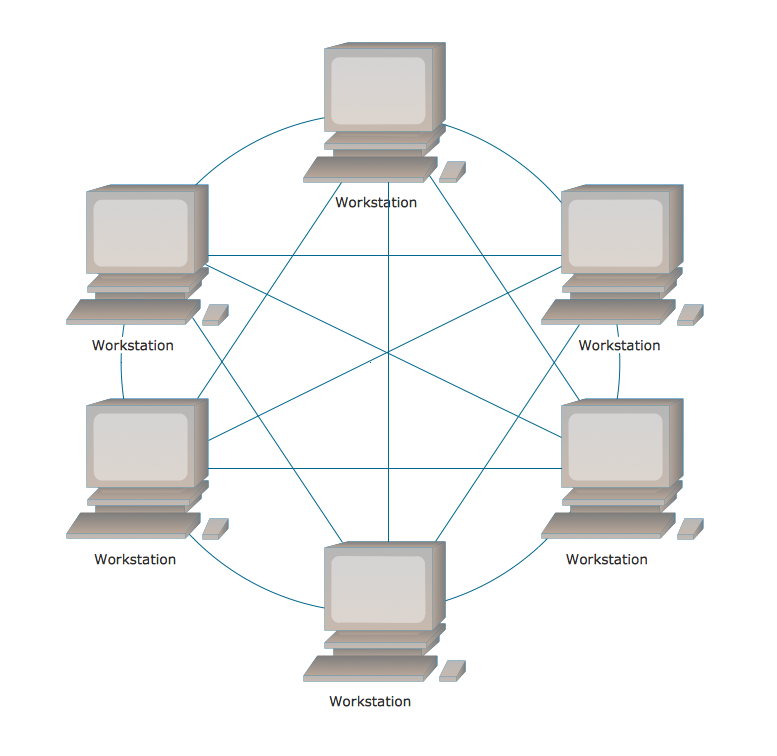
\includegraphics[width=25em]{network-direct}
				}
				\caption{Diagram of a Directly Connected Network}
				\label{fig:diagram-network-direct}
			\end{figure}
			
		&& \emph{Star network:} Network where devices communicate through a single, central device
			&&& See figure~\ref{fig:diagram-network-star} for a diagram
			
			\begin{figure}[!htb]
				\centering
				\href
				{http://starnetworking.weebly.com/}
				{
					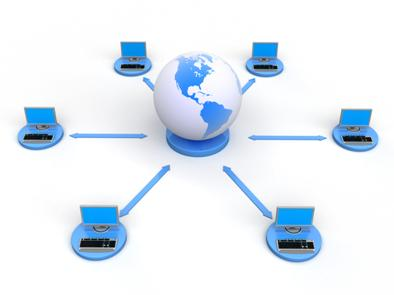
\includegraphics[width=25em]{network-star}
				}
				\caption{Diagram of a Star Network}
				\label{fig:diagram-network-star}
			\end{figure}
			
		&& \emph{Ring network:} Network where devices can communicate directly to two others in order to access another device, such that the devices are connected in a circle
			&&& See figure~\ref{fig:diagram-network-ring} for a diagram
			
			\begin{figure}[!htb]
				\centering
				\href
				{http://www.conceptdraw.com/examples/ring-network-topology}
				{
					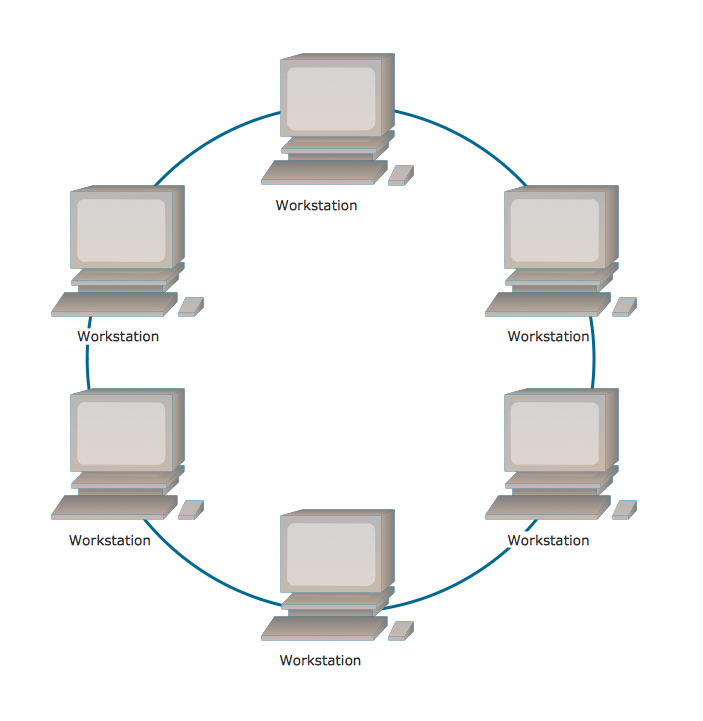
\includegraphics[width=25em]{network-ring}
				}
				\caption{Diagram of a Ring Network}
				\label{fig:diagram-network-ring}
			\end{figure}

\end{easylist}
\subsection{Internet Protocols}
	\label{subsec:networking:internet-protocols}
\begin{easylist}

	& World Wide Web:
		&& Collection of many networks
		&& Uses a network map to keep track of servers and their addresses
	
	& \emph{Socket address:} Unique identifier of a sender or receiver of data on the Internet, consisting of an \hyperref[subsec:networking:characteristics]{IP address} and a \hyperref[subsec:networking:characteristics]{port}
		&& When choosing a custom port in a computer application:
			&&& Common valid port numbers: 0 -- 65536
			&&& Ports reserved for other services: 0 -- 1024
			
	& \emph{User Datagram Protocol (UDP):} Internet communication protocol which is quick and lightweight
		&& Minimal protocol
		&& Does not require confirmation of connection or data transfer (no guarantee of reception)
		&& Order of data is not guaranteed
		&& Useful for time-sensitive information
		
	& \emph{Transmission Control Protocol (TCP):} Internet communication protocol which is reliable and error-checked
		&& Requires confirmation of connection and data transfer
		&& Order of data is guaranteed
		&& Data transmission adapts to the availability of the receiving buffer
		&& Can adapt to a congested network
		
\end{easylist}
\clearpage

	%
% IAT 267: Introduction to Technological Systems - A Course Overview
% Section: Arduino
%
% Author: Jeffrey Leung
%

\section{Arduino}
	\label{sec:arduino}
\subsection{Setup}
	\label{subsec:arduino:setup}
\begin{easylist}

	& Plug the Arduino into the computer
	& Open the Arduino IDE
	& Select the correct board and serial port
	& Verify and upload the program to the Arduino

\end{easylist}
\subsection{Physical Configuration}
	\label{subsec:arduino:physical-configuration}
\begin{easylist}

	& Figure~\ref{fig:arduino-uno-diagram} shows the layout of an Arduino Uno. \\
	The top pins are for digital input and output (and analog output, through \hyperref[sec:actuators]{PWM}). \\
	The bottom centre pins are for the standard power source and grounding. \\
	The bottom right pins are for analog input.

	\begin{figure}[!htb]
		\centering
		\href
		{https://www.element14.com/community/groups/arduino/blog/2014/12/17/rgb-led-shield-diagrams-for-documentation-purposes}
		{
			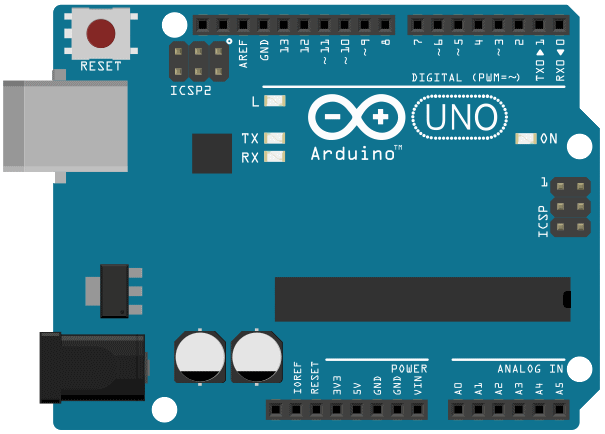
\includegraphics[scale=.5]{arduino-uno-diagram}
		}
		\caption{Arduino Uno Diagram}
		\label{fig:arduino-uno-diagram}
	\end{figure}

	& Uses an Atmel megaAVR \hyperref[subsubsec:electricity-and-circuit-design:circuits:components]{microcontroller}

	& Plugging in the USB cable provides power to the circuit

	& Power terminals:
		&& Positive: 5V
		&& Negative: GND (ground)

	& Switch:
		&& If the prongs are lined up vertically, the left prongs (top and bottom) are connected and the right prongs (top and bottom) are connected. When the button is pressed, the connection between the left pair and the right pair is bridged.
			&&& See figure~\ref{fig:arduino-switch} for an illustration of the prongs

			\begin{figure}[!htb]
				\centering
				\href
				{https://www.sparkfun.com/products/9190}
				{
					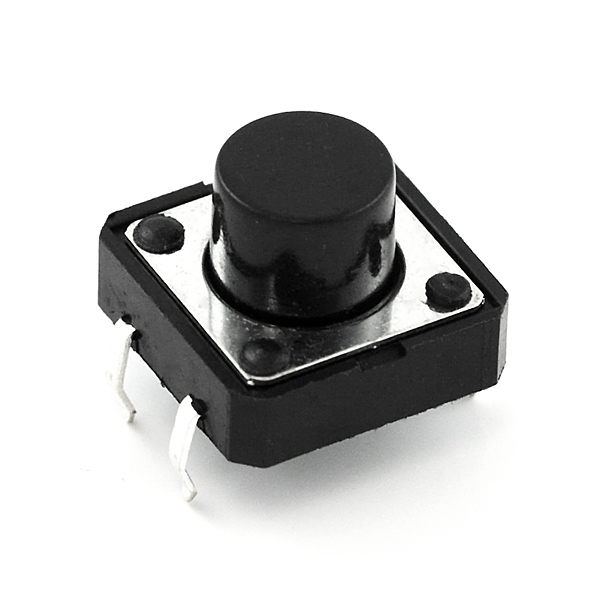
\includegraphics[scale=.3]{arduino-switch}
				}
				\caption{Momentary Pushbutton Switch. Activating the button bridges the two visible prongs.}
				\label{fig:arduino-switch}
			\end{figure}

	& Digital pin 13 has a built-in resistor

\end{easylist}
\subsubsection{Input/Output}
	\label{subsec:arduino:input-output}
\begin{easylist}

	& Digital input/output: Digital pins
		&& Can accept \textbf{HIGH} (5V) or \textbf{LOW} (0V)

	& Analog input: Analog pins
		&& Reads a value from 0 to 1023, proportional to the input voltage (0V to 5V)
		&& Uses an \hyperref[subsubsec:electricity-and-circuit-design:circuits:components]{analog-to-digital converter} in the Atmel megaAVR microcontroller in the Arduino
			&&& 6-channel
			&&& 10-bit resolution (1024 values)
		&& Requires a \hyperref[subsubsec:electricity-and-circuit-design:circuits:types-of-circuits]{voltage divider}

	& Analog output: Digital pins with the \textbf{\~{}} (tilde)
		&& Takes a value between 0 and 255, proportional to the amount of time that the voltage output is activated
			&&& Rapidly alternates between 0V and 5V
		&& All microcontrollers can only output a digital voltage, not an analog voltage
			&&& Uses \hyperref[sec:actuators]{pulse-width modulation} to simulate analog output

	& \hyperref[subsec:technological-systems:interaction]{Serial communication:}
		&& 8-bit communication
		&& \textbf{Serial.begin()} sets the data rate
		&& Digital pin 0 receives data (labeled RX)
		&& Digital pin 1 transmits data (labeled TX)
		&& \href{http://arduino.cc/en/Reference/Serial}{Arduino serial library}
		&& Only one program can receive serial input at a given time (e.g. Processing and the Arduino serial monitor cannot receive serial input at the same time)

\end{easylist}
\subsection{Programming}
	\label{subsec:arduino:programming}
\begin{easylist}

	& Arduino programming language:
	 	&& Set of C and C++ functions
		&& Compiled with \emph{avr-g++}
		&& Open source

	& \emph{Sketch:} Program written for an Arduino

	& \lstinline{void setup()}:
		&& Custom-defined function
		&& Run once before the other code
	& \lstinline{void loop()}:
		&& Custom-defined function
		&& Run continually
	& \lstinline{void serialEvent()}:
		&& Custom-defined function
		&& Executed after each iteration of the \lstinline{void loop()} function

	& Arduino libraries:
		&& \href{https://www.arduino.cc/en/Reference/Serial}{Serial}
		&& \href{https://www.arduino.cc/en/Reference/Servo}{Servo}
		&& \href{https://www.arduino.cc/en/Reference/softwareSerial}{SoftwareSerial}

\end{easylist}
\clearpage

	%
% IAT 267: Introduction to Technological Systems - A Course Overview
% Section: Processing
%
% Author: Jeffrey Leung
%

\section{Processing}
	\label{sec:processing}
\begin{easylist}

	& Processing programming language:
		&& Built upon Java
		&& Designed to create visually-oriented and interactive programs
		&& Open source

	& \lstinline[language=Java]{void setup()}:
		&& Custom-defined function
		&& Run once before the other code
		&& Window size: \lstinline[language=Java]{void size(x, y);}
		&& Background colour: \lstinline[language=Java]{void background(rgb);}
		&& Frame rate: \lstinline[language=Java]{void frameRate(frames);}
	& \lstinline[language=Java]{void loop()}:
		&& Custom-defined function
		&& Run continually

		& Coordinates begin at (0, 0) at the top left of the window
		& Colours set on the screen are additive

	& \href{https://processing.org/tutorials}{Official tutorials}
	& \href{https://processing.org/reference/libraries}{Processing libraries}
		&& \href{http://code.compartmental.net/tools/minim}{Minim (Audio)}
		&& \href{https://processing.org/reference/libraries/net}{Network}
		&& \href{http://processing.org/reference/libraries/serial}{Serial}

\end{easylist}
\clearpage


\end{document}
